\documentclass[journal,12pt]{IEEEtran}
\usepackage{graphicx} % Required for inserting images
\usepackage{mathpazo} % Palatino font
\usepackage{ragged2e} % Justification package
\usepackage{amsmath}
\usepackage{enumitem} % Enumerate in roman/alphabets etc
\usepackage{titlesec} % Edit section font 
\usepackage{tabularx} % Table with adjustable column width
\usepackage{tikz} % Required for creating diagrams
\usepackage{circuitikz}
\usetikzlibrary{shapes.gates.logic.IEC, positioning}
\renewcommand{\arraystretch}{1.5} % Adjust the value as needed

\titleformat{\section}{\normalfont\bfseries\filright}{\thesection}{1em}{\MakeUppercase}

\begin{document}
\onecolumn

\title{Platformio}
\author{\IEEEauthorblockN{Shreyas Kumar}}
\maketitle
\tableofcontents
\vspace{10pt}
\section{Question}
\vspace{10pt}
\begin{flushleft}
A Boolean function F of three variables X, Y, and Z is given as 
\vspace{3pt}
\\F(X, Y, Z) = (X' + Y + Z).(X + Y' + Z').(X' + Y + Z').(X' Y' Z' + X' Y Z' + X Y Z')\\
\vspace{3pt}
Which one of the following is true?
\end{flushleft}
\begin{enumerate}[label=\roman*.,labelindent=\parindent,leftmargin=*]
    \item F(X, Y, Z) = (X + Y + Z').(X + Y' + Z').(X' + Y' + Z')
    \vspace{1pt}
    \item F(X, Y, Z) = (X' + Y).(X + Y' + Z')
    \vspace{1pt}
    \item F(X, Y, Z) = (X' Z') + (Y Z')
    \vspace{1pt}
    \item F(X, Y, Z) = (X' Y' Z) + (X Y Z)
\end{enumerate}

\section{Solution}
\vspace{10pt}
\begin{flushleft}
F(X, Y, Z) = (X' + Y + Z).(X + Y' + Z').(X' + Y + Z').(X' Y' Z' + X' Y Z' + X Y Z') \\
\vspace{1pt}
\hspace{52pt} = (X' + Y + Z).(X + Y' + Z').(X' + Y + Z').(X' Z'.(Y + Y') + X Y Z') \\
\vspace{1pt}
\hspace{52pt} = (X' + Y + Z).(X + Y' + Z').(X' + Y + Z').(X' Z' + X Y Z') \\
\vspace{1pt}
\hspace{52pt} = (X' + Y + Z).(X + Y' + Z').(X' + Y + Z').(Z').(X' + X Y) \\
\vspace{1pt}
\hspace{52pt} = (X' + Y + Z).(X + Y' + Z').(X' + Y + Z').(Z').(X' + Y) \\
\vspace{1pt}
\hspace{52pt} = (X' + Y + Z).(X + Y' + Z').(X' + Y + Z').(Z').(X' + Y) \\
\vspace{3pt}
\textit{Let (X' + Y) = A} \\
\vspace{3pt}
F(X, Y, Z) = (A + Z).(X + Y' + Z').(A + Z').(Z').(X' + Y) \\
\vspace{1pt}
\hspace{52pt} = (X + Y' + Z').(A + ZZ').(Z').(X' + Y) \\
\vspace{1pt}
\hspace{52pt} = (X + Y' + Z').(X' + Y).(Z').(X' + Y) \\
\vspace{1pt}
\hspace{52pt} = (X + Y' + Z').(X' + Y).(Z') \\
\vspace{1pt}
\hspace{52pt} = (X' + Y).(XZ' + Z'Y' + Z'Z') \\
\vspace{1pt}
\hspace{52pt} = (X' + Y).(XZ' + Z'Y' + Z'Z') \\
\vspace{1pt}
\hspace{52pt} = (X' + Y).(XZ' + Z'Y' + Z') \\
\vspace{1pt}
\hspace{52pt} = (X' + Y).(Z').(X + Y' + 1) \\
\vspace{1pt}
\hspace{52pt} = (Z').(XX' + X'Y' + X' + YX + YY' + Y) \\
\vspace{1pt}
\hspace{52pt} = (Z').(X'Y' + X' + YX + Y) \\
\vspace{1pt}
\hspace{52pt} = (Z').(X'.(Y' + 1) + Y.(X + 1)) \\
\vspace{1pt}
\hspace{52pt} = (Z').(X' + Y) \\
F(X, Y, Z) = Z'X' + Z'Y
\end{flushleft}

\section{Truth Table}
\vspace{20pt}
\begin{center}
  \begin{tabularx}{0.46\textwidth} { 
  | >{\centering\arraybackslash}X 
  | >{\centering\arraybackslash}X 
  | >{\centering\arraybackslash}X
  | >{\centering\arraybackslash}X 
  | >{\centering\arraybackslash}X 
  | >{\centering\arraybackslash}X 
  | >{\centering\arraybackslash}X 
  | >{\centering\arraybackslash}X 
  | >{\centering\arraybackslash}X 
  | >{\centering\arraybackslash}X | }
\hline
\textbf{X} & \textbf{Y} & \textbf{Z} & \textbf{F}\\
\hline
0 & 0 & 0 & 1  \\  
\hline
0 & 0 & 1 & 0  \\ 
\hline
0 & 1 & 0 & 1  \\
\hline
0 & 1 & 1 & 0  \\
\hline
1 & 0 & 0 & 0  \\  
\hline
1 & 0 & 1 & 0  \\ 
\hline
1 & 1 & 0 & 1  \\
\hline
1 & 1 & 1 & 0 \\
\hline
\end{tabularx} \\
\vspace{6pt}
\textit{Truth table for Boolean function 'F' } 
\end{center}

\section{Logical Diagram}
\vspace{20pt}
\begin{center}
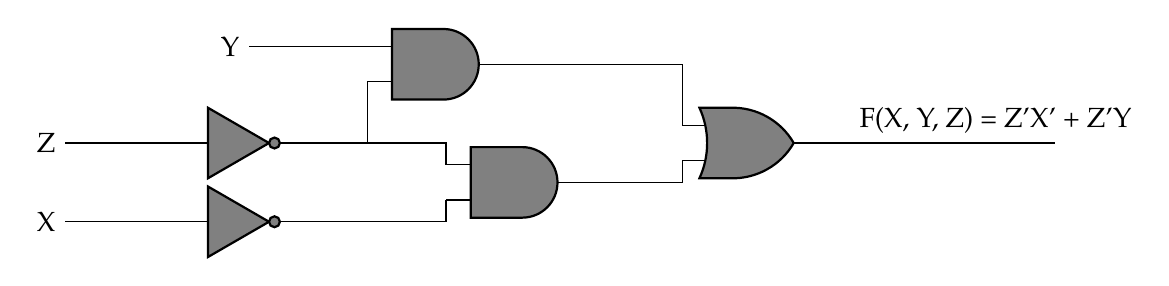
\begin{tikzpicture}
\ctikzset{
    logic ports=ieee,
    logic ports/scale=0.8,
    logic ports/fill=gray
}
 
% Logic ports
\node[not port] (nota) at (0,-2){};
\node[not port] (notb) at (0,-3){};

\node[and port] (anda) at (3.5,-2.5){};
\node[and port] (andb) at (2.5,-1){};
\node[or port]  (ora) at (6.5,-2){};
 
\draw (nota.out) -| (anda.in 1);
\draw (notb.out) -| (anda.in 2);
\draw (anda.out) -| (ora.in 2);
\draw (nota.out) -| (andb.in 2);
\draw (andb.out) -| (ora.in 1);

 
\draw (ora.out) -- ++(3,0) node[near end,above]{F(X, Y, Z) = Z'X' + Z'Y};
 
\draw (nota.in 1) -- ++(-1.5,0)node[left]{Z};
\draw (notb.in 1) -- ++(-1.5,0)node[left]{X};
\draw (andb.in 1) -- ++(-1.5,0)node[left]{Y};
 
\end{tikzpicture}
\end{center}

\section{Components}
\vspace{20pt}
\begin{center}
\begin{tabularx}{0.6\textwidth} { 
  | >{\centering\arraybackslash}X 
  | >{\centering\arraybackslash}X 
  | >{\centering\arraybackslash}X
  | >{\centering\arraybackslash}X | }
\hline
\textbf{Component} & \textbf{Values} & \textbf{Quantity} \\
\hline
Arduino & UNO & 1 \\
\hline
Jumper Wires & M-M & 10 \\
\hline
Breadboard & & 1 \\
\hline
LED & & 2 \\
\hline
Resistor & 220 ohms & 1 \\
\hline
\end{tabularx}
\vspace{6pt}
\\\textit{List of items required}
\end{center}

\section{Implementation}
\vspace{20pt}
\begin{center}
  \begin{tabularx}{0.46\textwidth} { 
  | >{\centering\arraybackslash}X 
  | >{\centering\arraybackslash}X 
  | >{\centering\arraybackslash}X  | }
\hline
\textbf{Arduino PIN} & \textbf{INPUT} & \textbf{OUTPUT} \\ 
\hline
\textbf 2 & X & \\
\hline
\textbf 3 & Y & \\
\hline
\textbf 4 & Z & \\
\hline
\textbf 13 & & F \\
\hline
\end{tabularx}
\vspace{6pt}
\\\textit{Connections}
\end{center}

\begin{flushleft}

Procedure:\\
\begin{enumerate}[label=\alph*.,labelindent=\parindent,leftmargin=*]
    \item Connect the circuit as per the above table.
    \vspace{2pt}
    \item Connect the output pin to LED.
    \vspace{2pt}
    \item Connect inputs to Vcc for logic 1, ground for logic 0.
    \vspace{2pt}
    \item Execute the circuit using the below code.
    \\
    \vspace{7pt}
    \begin{tabularx}{0.52\textwidth} { 
    | >{\centering\arraybackslash}X |}
    \hline
    https://github.com/shr-eyas/FWC/blob/main/platformio.cpp\\
    \hline
    \end{tabularx}
    \\
    \vspace{10pt}
    \item Change the values of X, Y, Z in the code and verify the truth table.\\
    
\end{enumerate}
\end{flushleft}

\bibliographystyle{ieeetr}
\end{document}
  
